\documentclass[tikz,border=2pt]{standalone}
\usepackage{amsmath}
\usepackage{pgfplots}
\pgfplotsset{compat=1.18}

\begin{document}
% Characteristic polynomial p(lambda) = (lambda-1)^2 (lambda-3) of a 3x3 matrix: the graph
% touches the axis at lambda = 1 (algebraic multiplicity 2) and crosses it at lambda = 3
% (multiplicity 1).
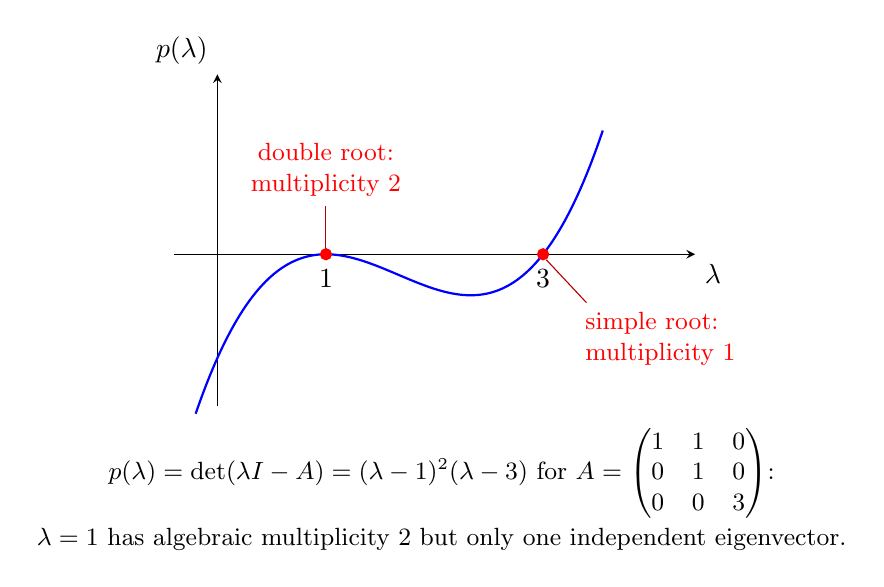
\begin{tikzpicture}
	\begin{axis}[
		axis lines=middle,
		xmin=-0.4, xmax=4.4, ymin=-2.2, ymax=2.6,
		xtick={1,3}, ytick=\empty,
		xlabel={$\lambda$}, ylabel={$p(\lambda)$},
		xlabel style={below right}, ylabel style={above left},
		samples=120, smooth, clip=false,
		width=8.2cm, height=5.8cm
		]
		\addplot[thick, blue, domain=-0.2:3.55] {(x-1)^2*(x-3)/2};
		\addplot[only marks, mark=*, red, mark size=2pt] coordinates {(1,0) (3,0)};
		\draw[red!70!black, thin] (axis cs:1,0.08) -- (axis cs:1,0.7);
		\node[red, anchor=south, font=\small, align=center] at (axis cs:1,0.7) {double root:\\ multiplicity $2$};
		\draw[red!70!black, thin] (axis cs:3.03,-0.08) -- (axis cs:3.4,-0.7);
		\node[red, anchor=north west, font=\small, align=left] at (axis cs:3.3,-0.7) {simple root:\\ multiplicity $1$};
	\end{axis}
	\node[anchor=north, align=center, font=\small] at (3.4,-0.15) {$p(\lambda)=\det(\lambda I-A)=(\lambda-1)^2(\lambda-3)$ for $A=\begin{pmatrix}1&1&0\\0&1&0\\0&0&3\end{pmatrix}$:\\[2pt] $\lambda=1$ has algebraic multiplicity $2$ but only one independent eigenvector.};
\end{tikzpicture}
\end{document}
